\section{Discussion and results}
\label{sec:discuss}

Time series of tidal water level and depth integrated currents are extracted using harmonic analyses on the both the observed and modelled time series. The eight major tidal constituents of diurnal (K$_1$ and O$_1$), semi diurnal (S$_2$, M$_2$, and N$_2$), and quarter diurnal (MN$_4$, M$_4$, and MS$_4$) frequencies are here evaluated and compared. 

In Run 1 (raw tidal forcing) the modelled amplitudes did not match the observed amplitudes and the maxima appeared too late in time (Fig.~\ref{fig:Viker_timeseries}). In Run 2 both phases and amplitudes improved as expected close to the open boundary (Table~\ref{tab:Viker}). The amplitudes of the principal lunar semidiurnal constituent (M$_2$) and its shallow water overtide (M$_4$) are increased, while the remaining are reduced. Likewise Tab.~\ref{tab:RMS} displays a dramatic decrease in the RMS error of the tides at Viker, from 5.4 cm (Run 1) to 2.3 cm (Run 2). A similar change in the correlation coefficient is also noteworthy from 0.85 to 0.97. The size of the adjustment factors and the change in the RMS error and correlation coefficient thus emphasise the need for adjustment of the tidal forcing at the boundary. 

Far from the southern boundary, we note that the RMS error at Oscarsborg is reduced, and even for the innermost Oslo station the RMS error is reduced (Tab.~\ref{tab:RMS}). A concomitant increase in the correlation coefficient is also evident. Table~\ref{tab:Oscarsborg} shows that the modelled tides have improved also in the inner parts of the fjord. 
The improvement is also evident in the scatter plots shown in Fig.~\ref{fig:Oslo_QQ_Scatter}. In particular we note the improvement regarding the tails, that is the maximum tides. 
Finally, the improvement in applying the adjusted tidal forcing is evident in the probability density distributions (PDFs) depicted in Fig.~\ref{fig:Oslo_PDF}. The observed tides at both Viker and Oscarsborg have a double peaked distribution, while the distribution of the tides in Run 1 only show one peak. Although not perfect, this two peak distribution is indeed achieved in Run 2, and hence is much more in line with the observed PDF. 

Since the modelled tides in the inner part of the fjord depend not only on the tidal forcing at the boundary, but also on how the propagation of the tidal waves are represented in the model, the improvement in the inner domain of the fjord is a crucial test of the method. As is well known, the ROMS model is a terrain-following model. Hence the topography and the irregular coastline of the model domain is smoothed and changed to minimise the ubiquitous pressure gradient error. In addition the smoothing is different in different parts of the domain due to the use of the curvilinear option. Thus the model's topography and irregular coastline do not necessarily reflect the true topology of the Oslofjord. Since the propagation speed $c$ of the tides depends crucially on a correct representation of the depth ($c = \omega/k \approx \sqrt{g h_c}$ where $g$ is the acceleration of gravity and $h_c$ is the characteristic depth), the remaining  discrepancies in the diurnal and quarter diurnal constituents indicate challenges that might be caused by a misrepresentation of the propagation. Finally, also possible errors in bottom friction may have an influence.

Fields of the amplitude and phase for M$_2$ reveal some interesting phenomena once the boundary forcing is adjusted (Fig.~\ref{fig:Oslofjord_tidal_fields}). The M$_2$ amplitude increases gradually northward from the open boundary in the south and all the way to the head of the fjord in the eastern branch. This can be explained by a progressive wave that propagates into the fjord and is reflected at the head. As observed, the sum of two progressive waves results in a wave with increasing amplitude in the northward direction. Although the representation of M$_2$ at the boundary is in good agreement with the observations, the representation at the innermost stations deteriorates somewhat.


\begin{figure}[!t]
\centering
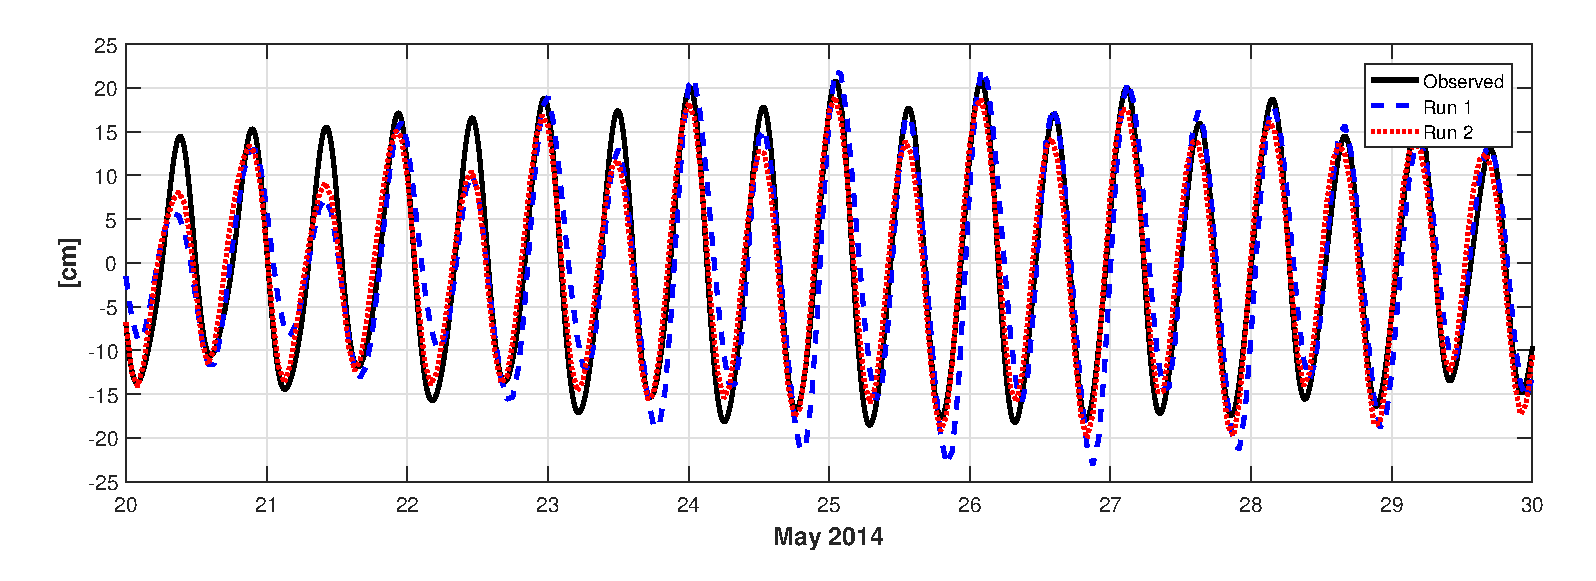
\includegraphics[width=\textwidth]{fig_Viker_timeseries}
\caption{Time series of tidal water level at a location close to Viker}
\label{fig:Viker_timeseries}
\end{figure}

\begin{table}[ht]
\caption{Tidal amplitudes [cm] and phases [deg] for the water level at Viker  together with adjustment factors $c^{(n)}$ and phase shifts $\triangle \phi^{(n)}$ for each component. The differences between modelled and observed values, are in parentheses.}
\label{tab:Viker}
\centering
\begin{tabular}{crrr@{ }lr@{ }lr@{ }lr@{ }lrr} \hline
      & \multicolumn{2}{c}{Observed} & \multicolumn{4}{c}{Run 1} & \multicolumn{4}{c}{Run 2} & \multicolumn{2}{c}{Adjustment} \\
Comp. & [cm] & [deg] & \multicolumn{2}{c}{[cm]} & \multicolumn{2}{c}{[deg]} & \multicolumn{2}{c}{[cm]} & \multicolumn{2}{c}{[deg]} & $c^{(n)}$ & $\triangle \phi^{(n)}$  \\ \hline 
S$_2$  &   3.0 &  39 &  5.1 & (2.1)  &  81 & (42)   &  3.2 & (0.2)  &  67 & (28)  &  0.588 &   -42.4   \\
M$_2$  &  11.8 & 105 &  9.7 & (-2.1) & 122 & (17)   & 11.8 & (0)    & 105 & (0)   &  1.224 &   -16.8   \\
N$_2$  &   3.4 &  57 &  5.7 & (2.3)  &  81 & (24)   &  3.1 & (-0.3) &  69 & (12)  &  0.595 &   -24.2   \\
K$_1$  &   0.7 & 136 &  1.2 & (0.5)  & 212 & (76)   &  0.1 & (-0.6) & 198 & (62)  &  0.554 &   -75.9   \\
O$_1$  &   2.2 & 279 &  3.7 & (1.6)  &  19 & (100)  &  2.9 & (0.7)  & 338 & (59)  &  0.591 &   259.8   \\
MN$_4$ &   0.4 & 263 &  1.0 & (0.6)  & 141 & (-122) &  0.3 & (-0.1) &   7 & (104) &  0.368 &   122.2   \\
M$_4$  &   1.2 & 275 &  0.7 & (-0.5) &  25 & (110)  &  1.1 & (0.1)  & 354 & (79)  &  1.742 &   249.2   \\
MS$_4$ &   0.3 & 348 &  1.1 & (0.8)  & 111 & (123)  &  0.6 & (0.3)  &  80 & (92)  &  0.272 &   236.7   \\ \hline
\end{tabular}
\end{table}

In the western branch of the fjord tidal choking occurs as water pass through the very narrow passage at the Svelvikstraum. Tidal chocking implies a decrease of tidal amplitude and a corresponding phase lag \cite[]{stigebrandt80} and occurs when the tidal wave enters a semi-enclosed basin through a sufficiently narrow inlet. This well-known phenomena is observed in several landlocked fjords and basins, for example Nord{\aa}svatnet and Saltfjord in Norway \cite[]{glenne63,eliassen01}, Mundau-Manguaba in Brazil \cite[]{oliveira93}, and Negembo Lagoon in Sri Lanka \cite[]{rydberg96}. 


\begin{table}[ht]
\caption{Tidal amplitudes [cm] and phases [deg] for the water level at Oscarsborg. The differences between modelled and observed values, are in parentheses.}
\label{tab:Oscarsborg}
\centering
\begin{tabular}{crrr@{ }lr@{ }lr@{ }lr@{ }l} \hline
      & \multicolumn{2}{c}{Observed} & \multicolumn{4}{c}{Run 1} & \multicolumn{4}{c}{Run 2}  \\
Comp. &  [cm] & [deg] & \multicolumn{2}{c}{[cm]} & \multicolumn{2}{c}{[deg]} & \multicolumn{2}{c}{[cm]} & \multicolumn{2}{c}{[deg]} \\ \hline 
S$_2$  &   3.6 &  59  &   6.1 & (2.5)  &  85 & (26)   &  3.7 & (0.1)  &  70 & (11)  \\
M$_2$  &  13.7 & 121  &  11.1 & (-2.6) & 128 & (7)    & 13.7 & (0)    & 111 & (-10) \\
N$_2$  &   3.9 &  74  &   6.6 & (2.7)  &  86 & (12)   &  3.6 & (-0.3) &  75 & (1)   \\
K$_1$  &   0.9 & 138  &   1.1 & (0.2)  & 213 & (75)   &  0.1 & (-0.8) &  44 & (-94) \\
O$_1$  &   2.4 & 281  &   3.9 & (1.5)  &  21 & (80)   &  3.1 & (0.7)  & 340 & (59)  \\
MN$_4$ &   0.6 & 308  &   2.0 & (1.4)  & 163 & (-145) &  0.5 & (-0.1) &  29 & (99)  \\
M$_4$  &   1.7 & 319  &   1.4 & (-0.3) &  44 & (95)   &  2.0 & (0.3)  &  15 & (56)  \\
MS$_4$ &   0.4 &  32  &   2.2 & (1.8)  & 135 & (103)  &  1.3 & (0.9)  & 106 & (74)  \\ \hline 
\end{tabular}
\end{table}

\begin{table}[ht]
\caption{RMS error and correlation coefficient for the tidal water level at the location of the three gauges in the model domain}
\label{tab:RMS}
\centering
\begin{tabular}{lrlrl} \hline
 & \multicolumn{2}{c}{RMS error} & \multicolumn{2}{c}{Correlation coefficient} \\ 
Station & Run 1 & Run 2 & \hspace{0.5cm} Run 1 & Run 2 \\ \hline 
Viker      & 5.4 &   2.3 &  0.82  &  0.97 \\
Oscarsborg & 5.8 &   3.3 &  0.85  &  0.95 \\
Oslo       & 6.0 &   4.9 &  0.85  &  0.90 \\ \hline
\end{tabular}
\end{table}

In coastal areas the currents vary both in time and over relatively short distances both vertically and horizontally. The currents at a position near Filtvedt were measured using a bottom-mounted profiling current meter from 18 September to 25 November 2014. The depth at the location of the observations was 167 meters. Due to noise in the upper levels of the observations, only depths below 40 meters depth are here included in the analyses. 

In order to compare observed and modelled tidal currents, harmonic analyses are performed on the depth averaged currents using T\_Tide.
Time series of the observed and modelled tidal currents are constructed based on the calculated tidal components for the time period of the observations (Fig.~\ref{fig:Filtvedt_timeseries}). The time series reveal that the amplitudes in Run 1 are too strong compared to the observations. 
An accurate representation of the currents at one specific position in shallow areas cannot be expected due to spatiotemporal challenges, but the tidal representation has improved after the adjustment (Table~\ref{tab:Filtvedt}). The RMS error decreased significantly and the correlation coefficient improved after the adjustments (Table~\ref{tab:RMS_currents}).

We conclude that the simple approach to adjust the tidal forcing gives improved and adequate accurate results for the area in question.


\begin{figure}[!t]
\centering
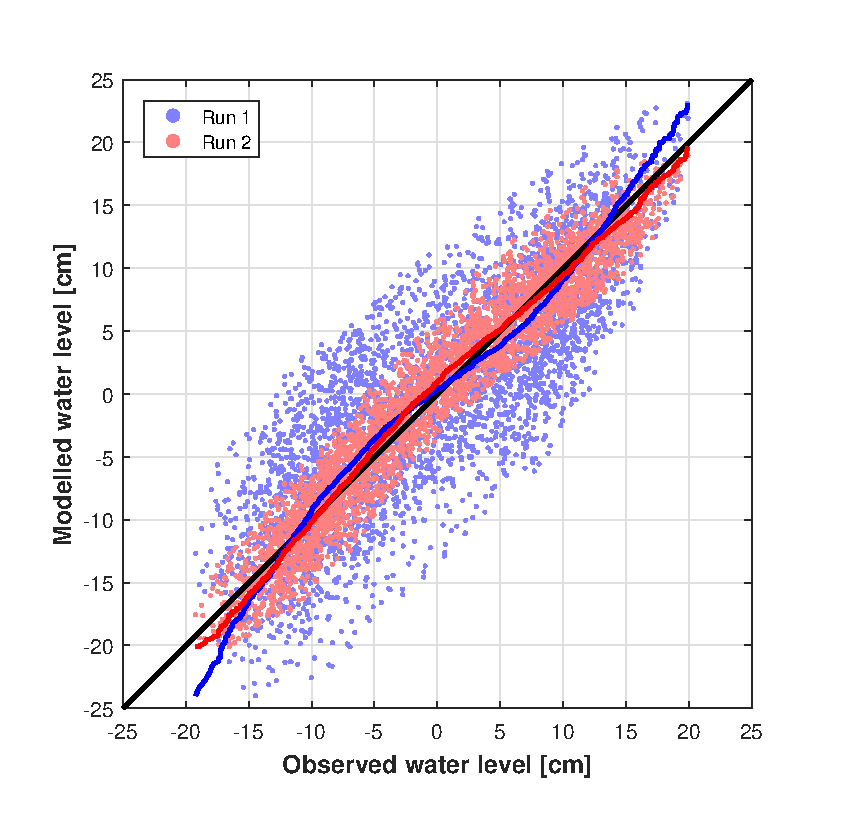
\includegraphics[width=0.49\textwidth]{fig_Viker_QQ_Scatter}
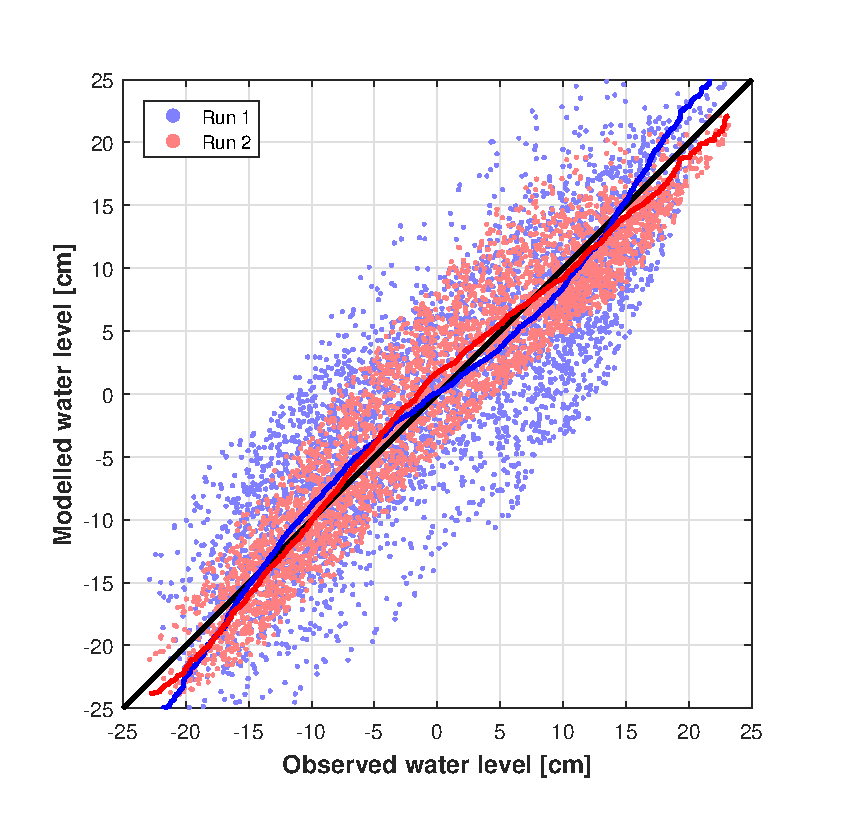
\includegraphics[width=0.49\textwidth]{fig_Oscarsborg_QQ_Scatter}
\caption{Combined QQ (solid) and scatter (dots) plot for the tidal water level at Viker (left) and Oscarsborg (right)}
\label{fig:Oslo_QQ_Scatter}
\end{figure}

\begin{figure}[!t]
\centering
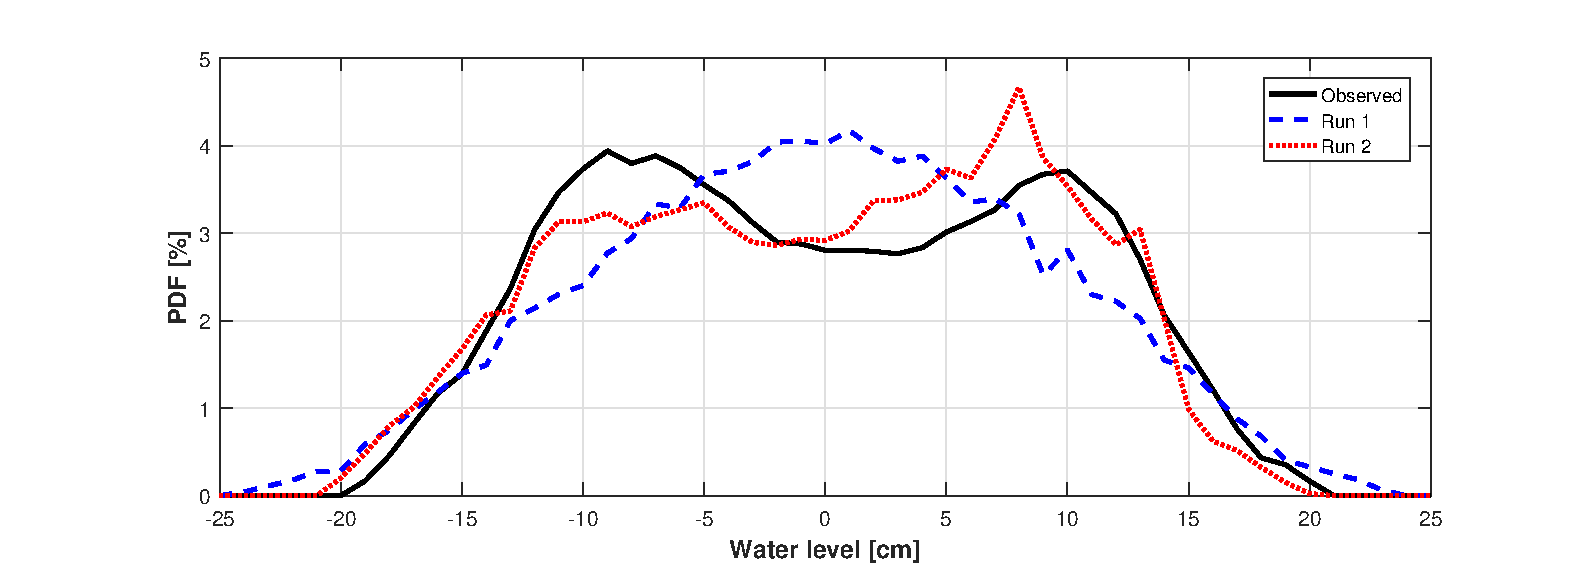
\includegraphics[width=\textwidth]{fig_Viker_PDF}
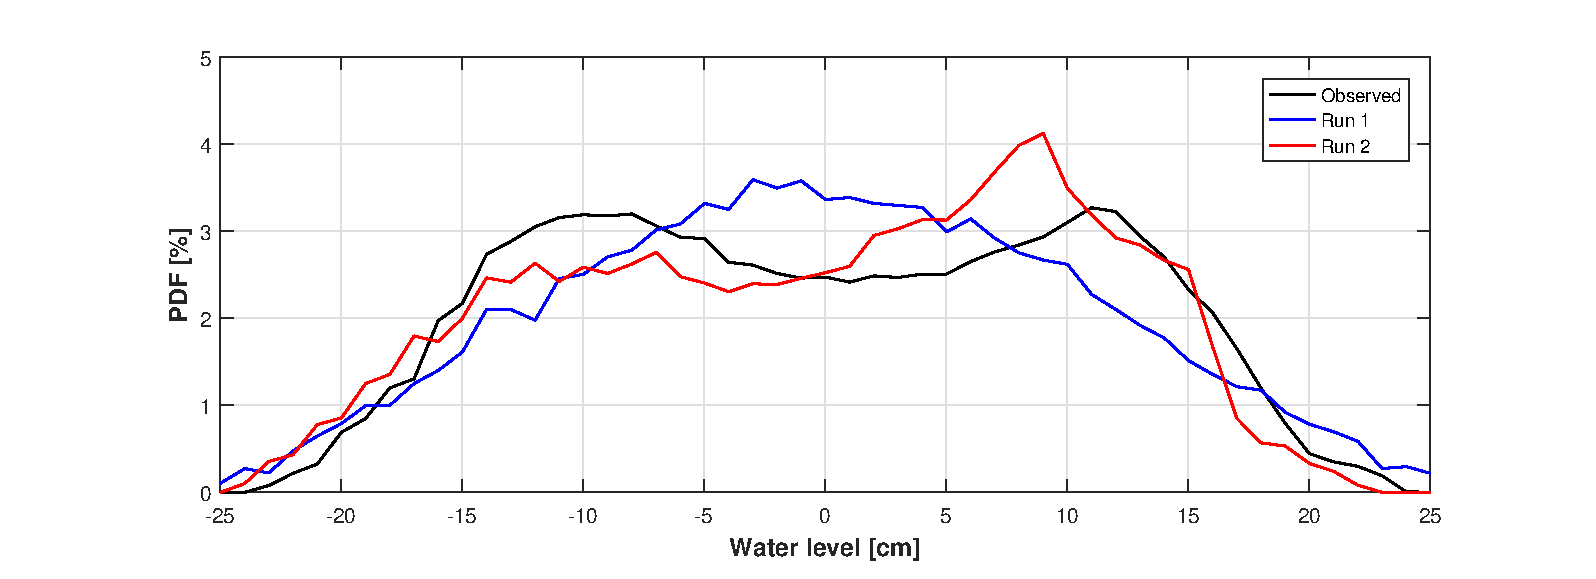
\includegraphics[width=\textwidth]{fig_Oscarsborg_PDF}
\caption{Probability density functions (PDF) for the tidal water level at Viker (upper) and Oscarsborg (lower). A bin size of 0.5 cm are applied on time series of the tidal water level. Since a ten minutes interval applies to the observations, the modelled time series are interpolated to time series with ten minutes intervals.}
\label{fig:Oslo_PDF}
\end{figure}


\begin{figure}[!t]
\centering
\includegraphics[trim=1cm 1cm 0cm 0cm,clip=true,width=0.49\textwidth]{fig_Oslofjorden_M2amp.eps}
\includegraphics[trim=1cm 1cm 0cm 0cm,clip=true,width=0.49\textwidth]{fig_Oslofjorden_M2phase.eps}
\caption{Fields of M$_2$ water level amplitude (left) and phase (right) based on run 2. The corresponding observed values are indicated by coloured circles at the three permanent gauges in the area.}
\label{fig:Oslofjord_tidal_fields}
\end{figure}


\begin{figure}[!t]
\centering
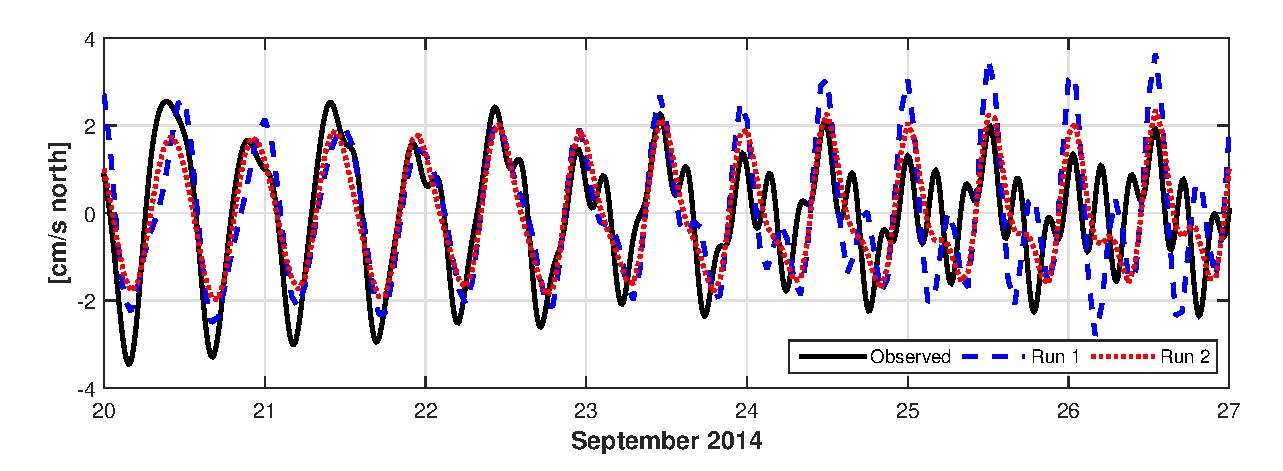
\includegraphics[width=\textwidth]{fig_Filtvedt_timeseries}
\caption{Time series of depth averaged tidal currents at a position close to Filtvedt. The time series are constructed based on the tidal components. Neither observed nor modelled currents at water depths less than 40 meters are included due to noise in the upper levels of the observations.}
\label{fig:Filtvedt_timeseries}
\end{figure}



\begin{table}[ht]
\caption{Tidal major amplitudes [cm/s] and phases [deg] for the depth integrated currents at a location close to Filtvedt}
\label{tab:Filtvedt}
\centering
\begin{tabular}{crrr@{ }lr@{ }lr@{ }lr@{ }l} \hline
      & \multicolumn{2}{c}{Observed} & \multicolumn{4}{c}{Run 1} & \multicolumn{4}{c}{Run 2} \\
Comp. & [cm/s] & [deg] & \multicolumn{2}{c}{[cm/s]} & \multicolumn{2}{c}{[deg]} & \multicolumn{2}{c}{[cm/s]} & \multicolumn{2}{c}{[deg]} \\ \hline 
S$_2$   &  0.5 & 280  &   1.4 & (0.9)  & 336 & (56)   &  0.5 & (0)    & 334 & (54)   \\ 
M$_2$   &  1.8 &   9  &   2.3 & (0.5)  &  18 & (9)    &  2.0 & (0.2)  &  16 & (7)    \\ 
N$_2$   &  0.5 & 293  &   1.3 & (0.8)  & 339 & (46)   &  0.5 & (0)    & 343 & (50)   \\ 
K$_1$   &  0.5 &  61  &   0.1 & (-0.4) &   5 & (-56)  &  0.0 & (-0.5) & 261 & (-160) \\ 
O$_1$   &  0.1 & 120  &   0.3 & (0.2)  & 244 & (124)  &  0.2 & (0.1)  & 250 & (130)  \\ 
MN$_4$  &  0.3 & 166  &   0.7 & (0.4)  &  52 & (-114) &  0.2 & (-0.1) & 305 & (139)  \\ 
M$_4$   &  0.7 & 220  &   0.6 & (-0.1) & 303 & (93)   &  0.7 & (0)    & 291 & (71)   \\
MS$_4$  &  0.0 & 252  &   0.8 & (0.8)  &  24 & (132)  &  0.4 & (0.4)  &  19 & (127)  \\ 
\hline 
\end{tabular}
\end{table}


\begin{table}[ht]
\caption{RMS error and correlation coefficient for the depth integrated tidal currents at a location close to Filtvedt}
\label{tab:RMS_currents}
\centering
\begin{tabular}{lrlrl} \hline
 & \multicolumn{2}{c}{RMS error} & \multicolumn{2}{c}{Correlation coefficient} \\ 
Station & Run 1 & Run 2 & \hspace{0.5cm} Run 1 & Run 2 \\ \hline 
Filtvedt   & 1.4 &   0.9 &  0.62  &  0.85 \\ \hline
\end{tabular}
\end{table}
